\documentclass{article}
\title{Improvement on Degrees of Truth Theory: Compute Degree of Truth by Taking Average of Truth Value Among All Contexts}
\author{Lu Xiaochuan}
\date{\today}
\usepackage{amsmath}
\usepackage{amssymb}
\usepackage{amsthm}

% \usepackage{booktabs}

\usepackage{graphicx}
\begin{document}
\maketitle

\begin{abstract}
	As a solution to the sorites paradox, degrees of truth theory is criticized generally because of the exact degree and location of borderlines is not computable. This essay will show one possible method for the computation. Under the assumption that there is single determined border for each context, average of truth among all contexts can be taken as contextual degree of truth, with computable borders and exact degree of truth.
\end{abstract}

\section{Background}

Sorites paradox says that, for a large amount $(A=n)$ of sands, which is certainly a heap, removing one sand won't turn this heap into non-heap, but by repeating this procedure by $n$ times, there will be no sand$(A=0)$, which is certainly a non-heap.

Use $H(A)$ to represent the heapness (degree of being a heap) of a certain amount, use $\equiv$ to represent being certain false or certain true. It's clear that $\exists{0<A_L<A_R}; H(A\leq A_L)\equiv 0, H(A\geq A_R)\equiv 1$.  Defining the maximum amount certain non-heap to be the left border$(A_L)$ and the minimum amount certain heap to be the right border$(A_R)$. The heapness of Amount in between are uncertain and needs further explaination.

Degrees of truth theory connects certain false and certain true by assigning each numbers between two borders a degree from 0 to 1, which ensures that truth values are continuous over $A \in [0, \infty)$. However, the degrees of truth theory is still unable to tell where the two borders$(A_L,A_R)$ locate and how the get the exact degree $H(A)$.

Contextualism, another theory for the sorites paradox, raised an assumption that for a given context$(c_i)$, there is a determined border$(A_i)$ between false and true. There are infinite contexts which generate infinite borders. This assumption is useful improving the Degrees of truth theory.

\clearpage

\begin{figure}[ht]
	\centering
	\begin{minipage}[t]{0.48\textwidth}
	\centerline{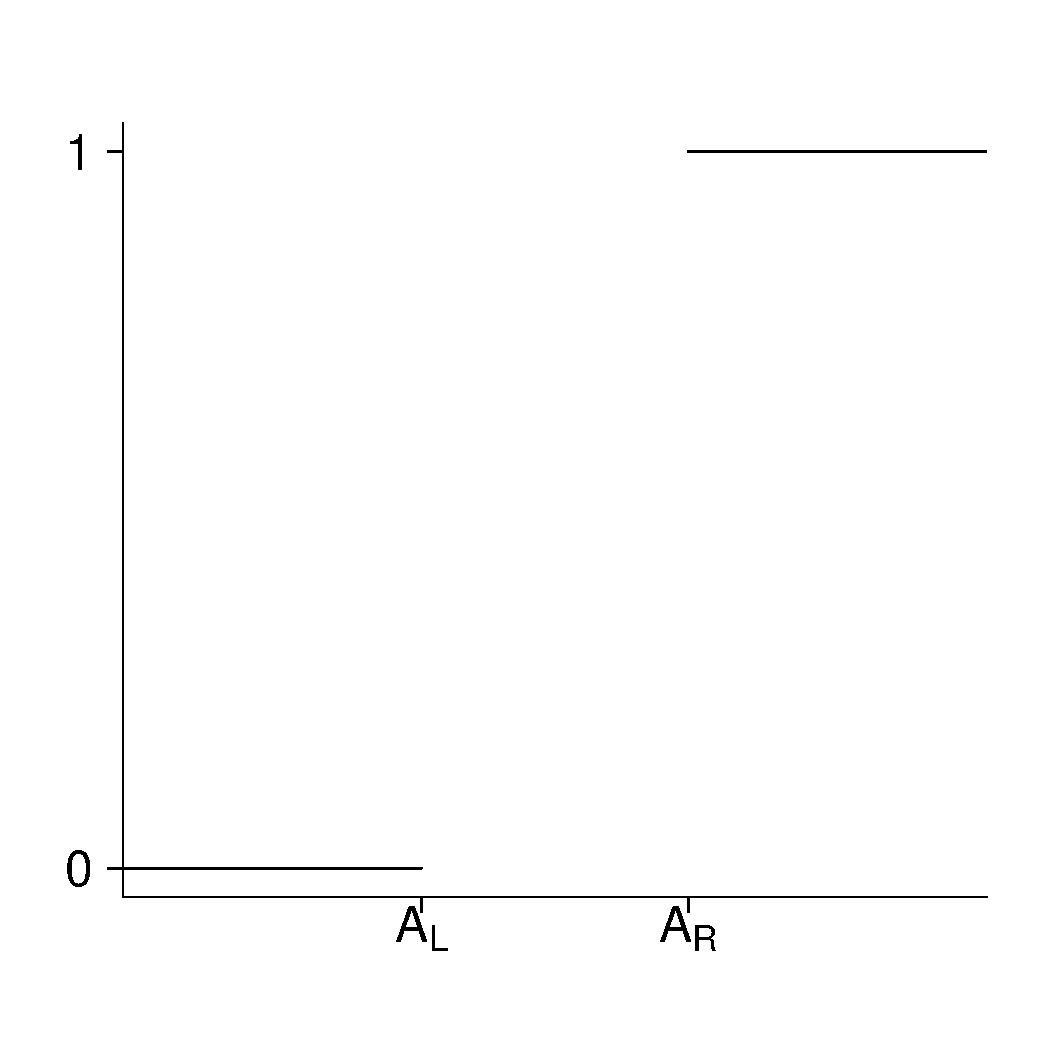
\includegraphics[scale=0.25]{plot1.pdf}}
	\caption{Certain heap and non-heap}
	\end{minipage}
	\begin{minipage}[t]{0.48\textwidth}
	\centerline{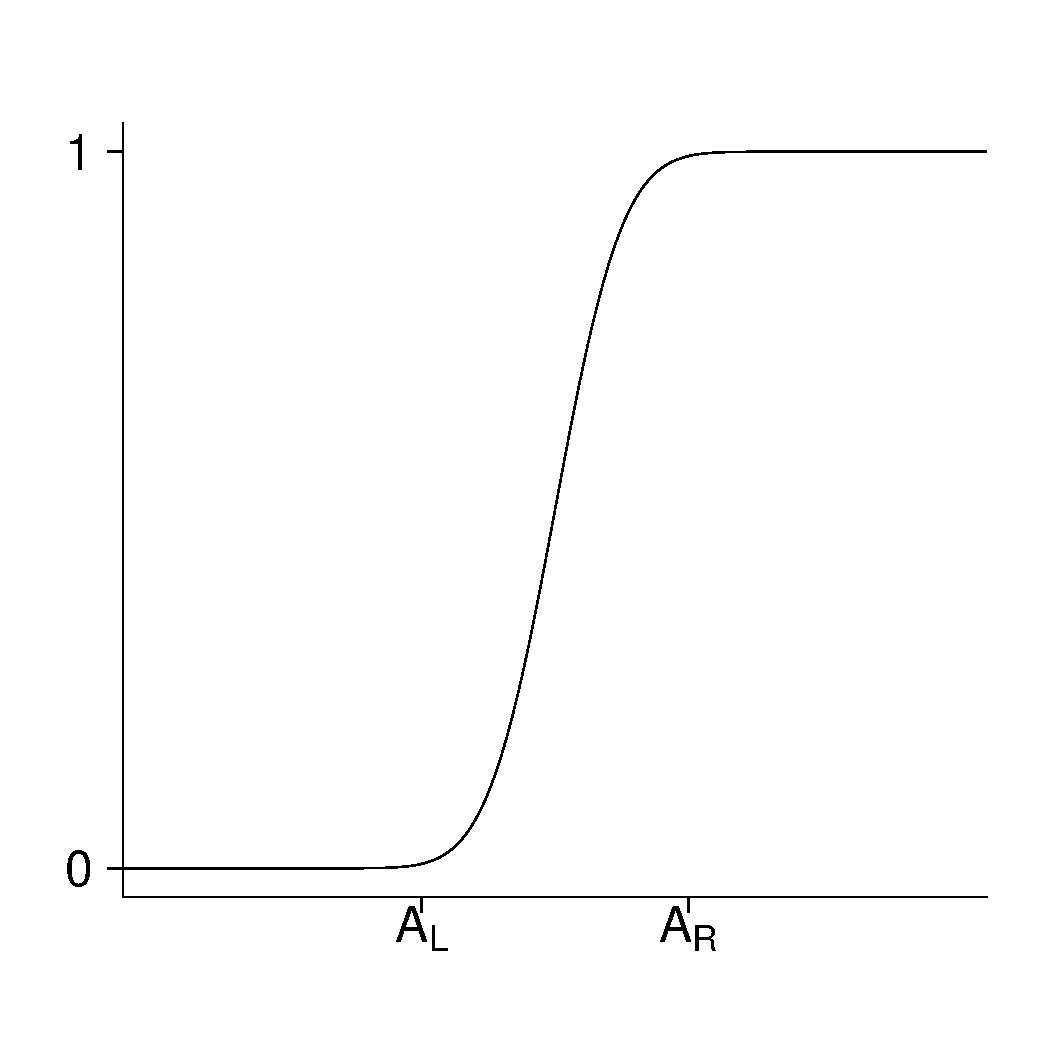
\includegraphics[scale=0.25]{plot3.pdf}}
	\caption{Degree of truth theory}
	\end{minipage}
\end{figure}

\section{Model}

Assuming that in a given context$(c_i)$, there is a single determined border$(A_i)$ from non-heap to heap. Use $\Rightarrow$ to represent determine, $A_i$ can not be changed unless $c_i$ is changed.
\[c_i\Rightarrow A_i, where\ \forall A<A_i,H(A)=0;\forall A>A_i,H(A)=1\]

\begin{enumerate}
\item The judge is unchangeable in the context.
\item The criteria should ensure that only true and false are output.
\end{enumerate}

E.g. Amount of sand required to build a building, if the building works without any problem, then this amount forms heap in context, otherwise it's not.

When we face a "context" in the real life, it does not meet the $c_i\Rightarrow A_i$ assumption, we can use case($C$) to represent it. $C$ contains a set of contexts that have determined border, and it's impossible to identify the exact context from this set.

\[C=\{c|c=c_0+offset\}\]

\begin{figure}[ht]
	\centering
	\begin{minipage}[t]{0.48\textwidth}
	\centerline{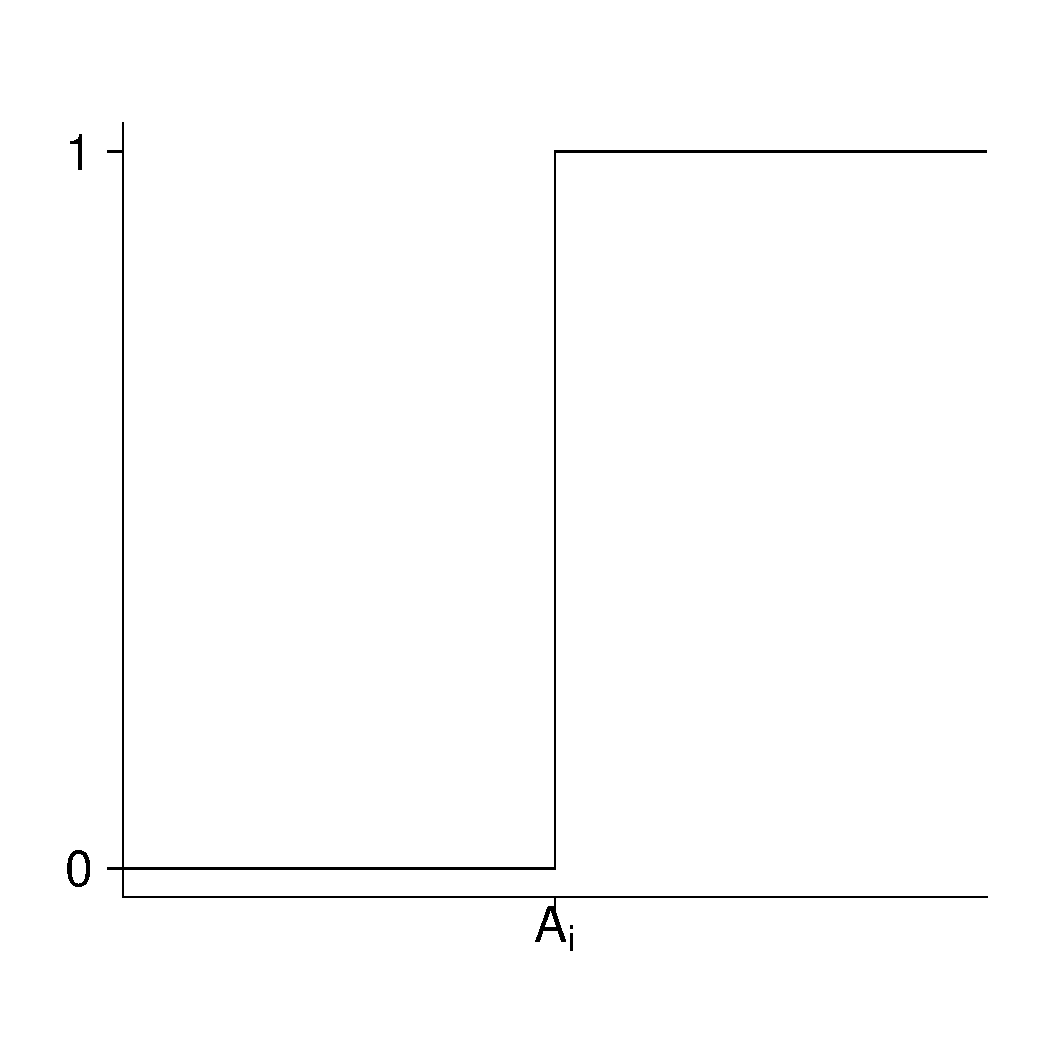
\includegraphics[scale=0.25]{plot2.pdf}}
	\caption{Single context$(c_i)$}
	\end{minipage}
	\begin{minipage}[t]{0.48\textwidth}
	\centerline{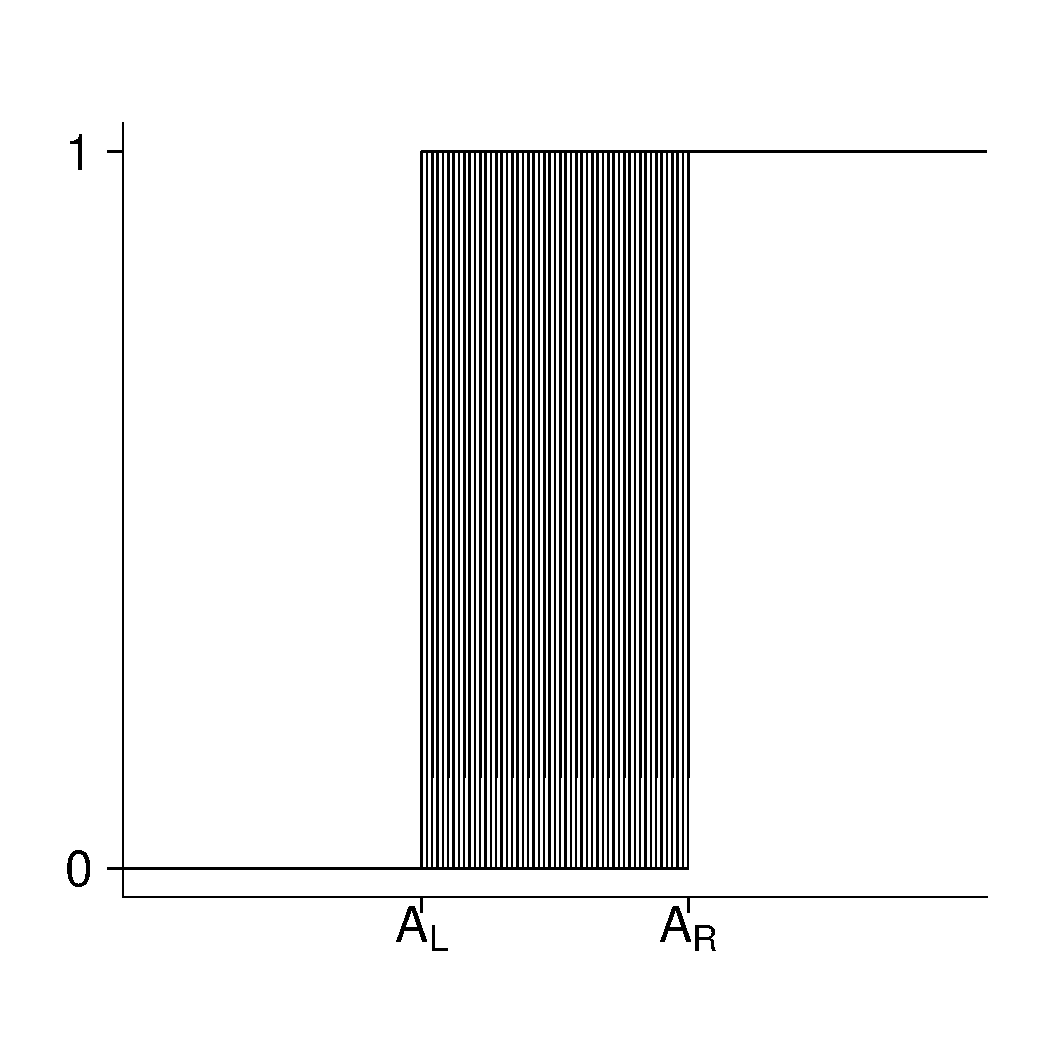
\includegraphics[scale=0.25]{plot4.pdf}}
	\caption{case$(C)$ in real life}
	\end{minipage}
\end{figure}

\subsection{Taking average}
Since there is a set of contexts, Truth in single context$(H(A)|c_i)$ can be computed by comparing the amount$(A)$ with border of each context$(A_i)$. The average of truth among all contexts can be taken, the result is the probability of being heap among the context set. The resulted curve has the same monotonicity and continuity described in the the degree of truth theory, and it can be called contextual degrees of truth:

\[H(A)|C=\lim_{n\to \infty}\frac{1}{n}\sum_{i=1}^{n}H(A)|c_i; c_i\in C\]

The more accurate version, $m=\int_C 1$, as the mass of the set:
\[H(A)|C=\frac{1}{m}\int_C H(A)\]

$A_L=\min(A_i),A_R=\max(A_i)$. $H(A)|C = P[(H(A)|c_i) = 1]$.

\section{Justification}

% Assumption make sure no vageness in single context
The only assumption added in this improvement is $c_i\Rightarrow A_i$. In this assumption, the context is well-defined and would always be binary. There should be no vagueness in single context. When using the contextual degree of truth, the case should be decomposed that each element is strict context.

% context set always come together
When judging whether a object fit the criteria of the term, as long as it's a vague term, either judge is changeable or the criteria can produce a indeterminate truth value. When we face a context strictly satisfied the assumption. E.g.\ An individual is defined to be an adult when $age\geq 18$. The context here strictly satisfied the assumption, but it is not vague anymore, even if it use the same word with adult in other contexts. Therefore, context for vague term won't appear alone.

% Why studying context set is neccesary
Contextualism is based on the assumption of $c_i\Rightarrow A_i$. When judging the difference of two amount beside the border $(A_i\pm 1)$. It just answered context has changed when focusing around the borderline. In other words, the judging object$(A)$ can change the judge's attitude. It might be a effective explain but also a unsatisfactory one. If context stay constant, removing sand at the borderline can suddenly change a heap into non-heap, but the situation for the sudden change does not exist because $A$ is changing as sand is removed. To explain the indifference in removing sand, a set of contexts exist simultaneously, and it's necessary to study on the set of contexts as a combination.

% Overcome Infinty
Some may worry that average of heapness among infinite contexts is uncomputable. Calculating the average among an infinite uncountable set is similar to calculating the expectation of a continuous distribution. The only difference is that each element in a distribution of statistics is a real number, while each element in the set $C$ is a context, determining the $H(A)$ function. $A$ and $H(A)$ are all real number. For Each $A$, the probability of being true can be measured, and the $H(A)|C$ is the combination for each $A$. 

\section{Discussion \& Conclusion}

By introducing the single context generate single determined border assumption, degree of truth theory can be improved as contextual degree of truth theory, which explains how the degree of truth for each amount comes from: Degree of Truth is the probability of being true among the context set. Contextual degree of truth has consistency with individual's belief, and can be illuminating studying the convergence of belief in communication. The improved theory reveals that the vagueness depends on the variation of contexts. The study on the distribution of truth is shifted to the distribution of contexts. This theory also gives guidance to the fuzzy logic that it could obey the rule both in probability theory and set theory.
\end{document}
